\documentclass[fleqn,usenatbib,twocolumn]{mnras}
\usepackage[utf8]{inputenc}
\usepackage{graphicx}
\usepackage{mathtools}
\usepackage{siunitx}
\usepackage{enumerate}
\usepackage{caption,subcaption}
\usepackage{comment}
\captionsetup{compatibility=false}
\usepackage{animate}
\usepackage{amsmath} % For \text and many other math symbols
\usepackage{amssymb} % For \mathbb
\usepackage{amsfonts} % For \mathbb
%%%%%
\usepackage{color}
\definecolor{RED}{rgb}{1,0,0}
\definecolor{BLUE}{rgb}{0,0,1}
%\usepackage[normalem]{ulem}
\usepackage{soul}
\usepackage{ulem}
\usepackage{comment}

\newcommand{\abs}[1]{\left|#1\right|}
\newcommand{\norm}[2]{\left\lVert#1\right\rVert}

\title{Image reconstruction of stellar objects with Intensity Interferometry using Generative Adversarial Networks}
\date{}

\begin{document}
\maketitle

\begin{abstract}
In modern astronomy, simulations of Intensity Interferometry are making significant strides in achieving high-precision resolution of stellar objects at optical wavelengths. Despite these advancements, phase retrieval remains a major challenge due to the nature of photon correlation. This paper explores the application of a conditional Generative Adversarial Network (GAN) to tackle the problem of image reconstruction in Intensity Interferometry. The proposed GAN-based approach effectively reconstructs the shape, size, and brightness distribution of a fast-rotating star by leveraging sparsely sampled, phase-subtracted Fourier transforms of the source. This method not only enhances the image reconstruction capabilities of Intensity Interferometry but also enables precise parameter estimation in astronomical observations.  
\end{abstract}
\section{Introduction}

Intensity Interferometry (II) was first reported by Hanbury Brown and Twiss (HBT) during the 1950s \citep{brown1954lxxiv, HBT56} as a \textquotedblleft new type of interferometry\textquotedblright\ to measure stellar parameters such as angular diameter, orbits, and limb darkening coefficients. Later, theoretical results reported by \cite{brown1957interferometry, brown1958interferometry}, along with those of \cite{glauber1963quantum} and others, demonstrated the deeper physical properties of photon correlations that lie at the core of II and laid the foundation for Quantum Optics \cite[for textbook treatments see][]{MandelWolf1995, Hecht2002}.

By the 1970s, with stellar parameter measurements of 32 stars in single and multiple star systems conducted by Hanbury Brown and his collaborators \citep{hanbury1974angular} at the historic Narrabri Stellar Intensity Interferometer (NSII) in Australia, II had emerged as an alternative to the already established technique of Michelson Interferometry for measuring stellar parameters. Despite these significant achievements, the method did not gain widespread adoption in the ensuing decades, primarily due to the unavailability of sensitive photon detectors and advanced data analysis equipment.

More recently, proposals emerged to utilize Imaging Atmospheric Cherenkov Telescope (IACT) facilities for conducting II observations of stars \citep{LeBohec2006, nunez2010stellar, nunez2012high, 2013APh....43..331D}. It was suggested that such observations could be carried out during bright, moonlit nights when $\gamma$-ray observations based on upper atmospheric Cherenkov showers were not feasible. This approach has the potential to enhance the scientific output of existing IACT facilities, and especially of the upcoming Cherenkov Telescope Array Observatory (CTAO).  SII observations at VERITAS, MAGIC, and HESS are now appearing \citep[e.g.,][]{2024ApJ...966...28A,2024MNRAS.529.4387A,2025MNRAS.537.2334V}. Simulations \citep[e.g.,][]{10.1093/mnras/stab2391, 10.1093/mnras/stac2433} have argued that recent advancements in photon detectors could be effective in achieving high-precision measurements of parameters for stellar objects. 

Beyond measuring stellar diameters and other parameters of star systems, a fundamental goal of optical astronomy is to image stellar systems at high angular resolution.  In the context of II, this involves reconstructing the source's image from the intensity correlations recorded by pairs of telescopes (light buckets) on the ground. However, because the primary observable in II is the electromagnetic field intensity rather than the field amplitude, the phase of the interferometric signal is lost. Since a complete reconstruction of a source's brightness distribution requires phase information, the challenge is to recover the phase of the signal.

Several theoretical and computational approaches for phase reconstruction with II have been proposed. \cite{gamo1963triple} introduced the concept of triple-intensity correlation, which \cite{goldberger1963use} subsequently applied in an experiment to observe scattered particles in microscopic systems. Sato conducted experiments to measure the diameter and phase of asymmetrical objects, suggesting that triple correlation could extend II to image stellar bodies \citep{sato1978imaging, sato1979computer, sato1981adaptive}. However, achieving a satisfactory signal-to-noise ratio (SNR) remained a significant challenge for this approach.

\cite{GerchbergSaxton1972} suggested an iterative method to determine the phase from the image and diffraction plane pictures. This method relies on accurate initial estimates and may struggle with slow convergence otherwise. \cite{Fienup1982} introduced a Hybrid Input-Output algorithm that incorporates feedback mechanisms to improve convergence rate and robustness, particularly in noisy environments.

Later, \cite{holmes2010two} proposed an alternative method that utilizes the Cauchy-Riemann relations to reconstruct 1-D images and extends the approach to 2-D images across a range of signal-to-noise (SNR) values. This algorithm was applied to simulated data of stellar objects using II, considering both existing and forthcoming Imaging Cherenkov Telescope Arrays (IACTs) with a large number of telescopes \citep{nunez2010stellar, nunez2012high, nunez2012imaging}. However, this method faces challenges related to computational complexity when attempting to generalize to higher dimensions.

\cite{Li2014} suggested a flexible iterative Regularization method that incorporates prior information (e.g., sparsity, smoothness, or non-negativity) to reduce the ill-posedness of the phase retrieval problem. This method is more robust against noise and stabilizes the solution against artefacts and spurious solutions. Nevertheless, it faces challenges regarding the choice of the regularization parameter, computational complexity, and sensitivity to the initial guess.

The Transport-of-Intensity Equation (TIE) method is a non-interferometric technique first proposed by \cite{Teague1983} that relates the intensity variations along the optical axis to the phase of the optical fields. This method enables phase retrieval from intensity measurements taken at multiple planes. \cite{Zhang2020} proposed a method to obtain a \textquotedblleft universal solution\textquotedblright\ to the TIE by employing a \textquotedblleft maximum intensity assumption\textquotedblright, thereby converting the TIE into a Poisson equation which is then solved iteratively. More recently, \cite{Kirisits2024} explored hybrid methods that combine the TIE with other equations, such as the Transport of Phase Equation (TPE). These approaches leverage the strengths of both equations to improve phase retrieval accuracy. This method is universally applicable, as it works for arbitrarily shaped apertures, handles non-uniform illumination, and accommodates inhomogeneous boundary conditions. It guarantees convergence, although the speed of convergence depends on the quality of the initial guess, and the final results are influenced by the boundary conditions.

With non-linearity built into their architecture, artificial neural networks (ANNs) empowered by deep learning methods are promising for exploring the task of reconstructing images of stellar objects from ground-based observations. Convolutional Neural Networks (CNNs), with their specialized architecture for processing two-dimensional datasets, are a natural choice for image processing tasks. In astronomical image reconstruction projects, a common challenge is that the interferometric data are typically undersampled as well as noisy.  Therefore, the CNN architectures and deep learning methods employed must be capable of reliably learning both the global context of the training dataset and the local features within it. Among the various CNN architectures, U-Net models \citep{ronneberger2015u} have proven successful in such tasks.

Furthermore, given that achieving a high signal-to-noise ratio (SNR) is often challenging in astronomical datasets, it is immensely beneficial if additional data can be generated using the available information from the observed sky density distribution and ground-based observations (II data, in our case) of the sources under investigation. Generative Adversarial Networks (GANs), introduced by \cite{goodfellow2014generative}, have been successful in data augmentation tasks. Conditional GAN (cGAN) architectures, proposed by \cite{mirza2014conditional} and applied to a wide variety of datasets by \cite{isola2017image}, leverage additional information about the images in the training datasets and have demonstrated remarkable robustness in image recovery across diverse data types.

In the astrophysical context, \cite{schawinski2017galaxypics} employed a GAN model to recover features—such as spiral arms, central bulges, and disk structures—of galaxies from noise-affected images. \cite{mustafa2019cosmogan} developed and customized a Deep Convolutional GAN, dubbed \textquotedblleft CosmoGAN\textquotedblright, capable of generating high-fidelity weak-lensing convergence maps of the dark matter distribution that statistically reproduce real weak lensing structures. \cite{coccomini2021lightweightgan} have successfully generated credible images of planets, nebulae, and galaxies using \textquotedblleft lightweight\textquotedblright\ and \textquotedblleft physics-uninformed\textquotedblright\ GANs to produce synthetic images of celestial bodies. They also generated a \textquotedblleft Hubble Deep Field-inspired\textquotedblright\ wide-view simulation of the universe. 

In this paper, we propose a conditional Generative Adversarial Network (cGAN) model \citep[following][]{isola2017image} to reconstruct images of fast-rotating stars using their simulated Intensity Interferograms and simulated sky-intensity distributions as input data for training, testing, and validation. We consider four Imaging Cherenkov Telescope Arrays (IACTs) and simulation observation of a fast-rotating star. The image predicted by the trained GAN shows promising results in reconstructing the star’s shape and size. The reconstructed brightness distributions are then assessed using moments.

This paper is organized as follows. The next section discusses Intensity Interferometry, focusing on its signal and noise characteristics for fast-rotating stars along the Earth’s rotation. The following section introduces the GAN formulation and its structure. The fourth section details the parameter selection for training the GAN for image reconstruction. The fifth section presents the results of the trained GAN both visually and via image moments. Finally, the paper concludes with a discussion of the overall results.
\begin{figure}[hbt]
	\centering
	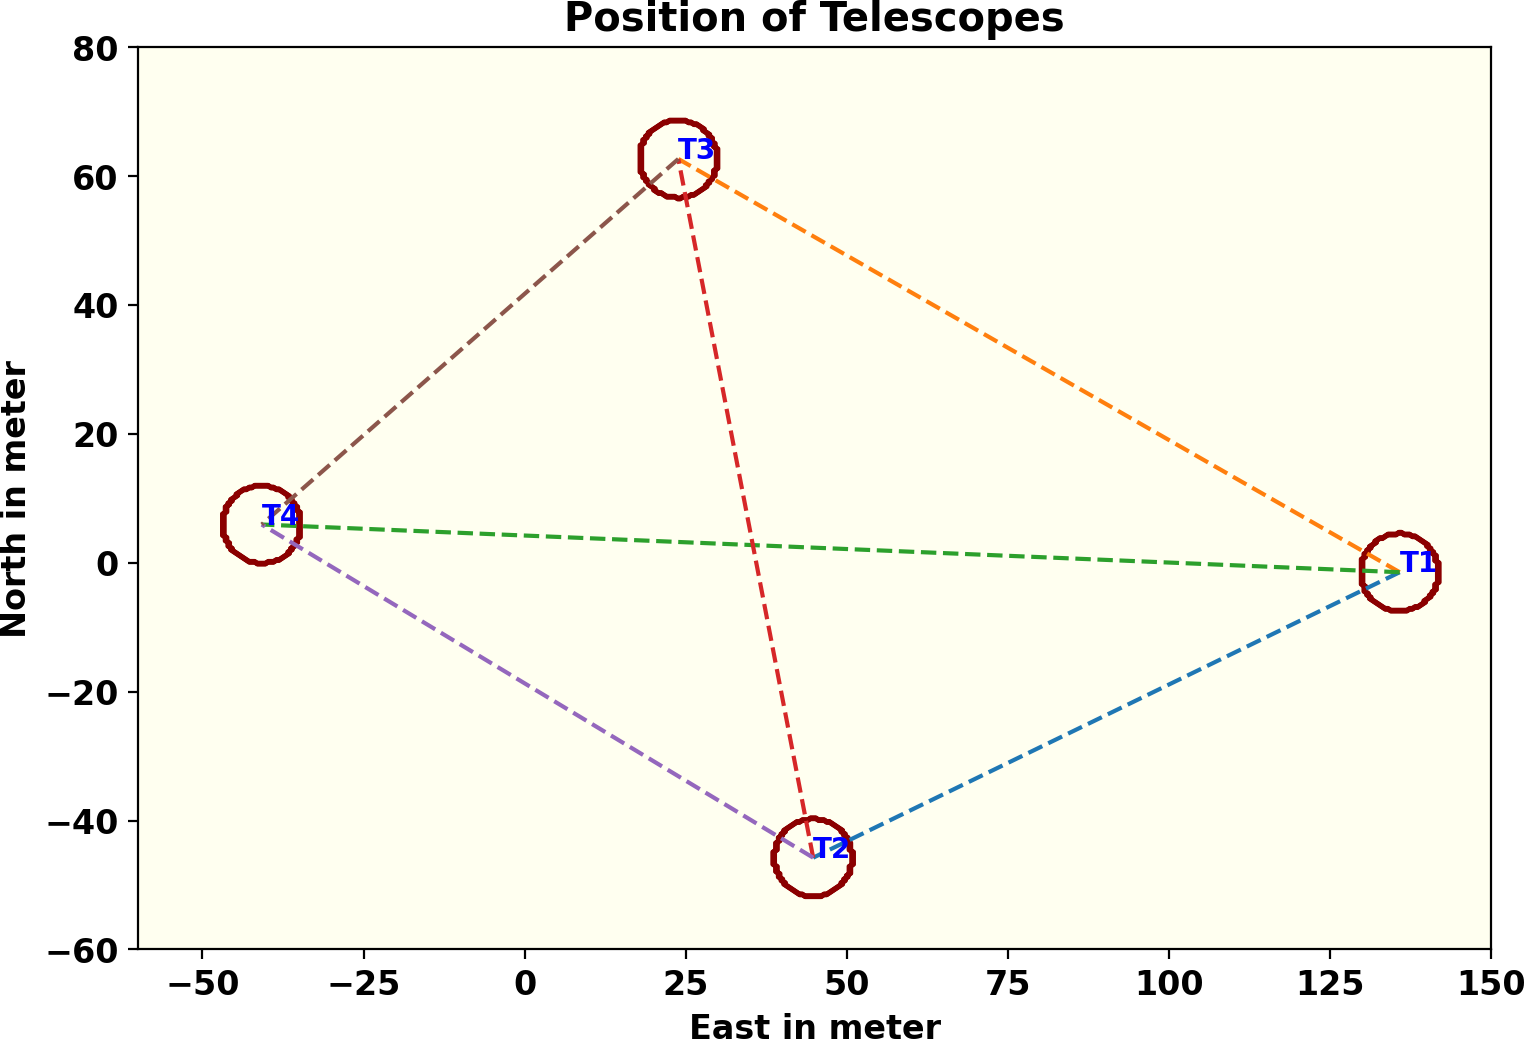
\includegraphics[width=\linewidth]{fig/telescope.png}
	\caption{The telescope configuration with similar properties each used to simulate the signal for II.}
	\label{fig:teles}
\end{figure}
\section{Intensity Interferometry (II) with IACT arrays}
R. Hanbury Brown and Robert Q. Twiss (HBT) carried out the first experiments demonstrating the possibility of measuring angular diameter of stars using Intensity Interferometry (II) in optical wavelengths \citep{HBT56}. Subsequently, they also pioneered the theoretical background of II and conducted laboratory experiments \citep{brown1957interferometry,brown1958interferometry},thereby further consolidating II as an alternative method, besides the already established Michelson Interferometry, to measure stars. Further, HBT also successfully installed the Narrabri Stellar Intensity Interferometer \textcolor{blue}{during the 1960s-70s and successfully used it to measure the angular diameters of bright stars in the spectral range $\mathrm{O5f}\ -\ \mathrm{F8}$ using visible wavelengths} signals \citep{brown1974intensity}. \\\textcolor{blue}
{However, the available speed and sensitivity of electronics in the 1970s was not favourable for more extensive and larger scale measurement projects using II.}

\textcolor{blue}{Subsequently, during the opening decades of the current century, proposals to use the Imaging Atmospheric Cherenkov Telescope (IACT) facilities for carrying out Stellar Intensity Interferometry (SII) observations were put forth \citep{LeBohec2006, nunez2010stellar, nunez2012high, Dravins2013}. Such observations, it was suggested, could be carried out during bright moon-lit nights during which $\gamma$-ray observations using upper atmospheric Cherenkov showers were not feasible. This idea had the potential of enhancing the scientific output of the existing facilities like VERITAS, MAGIC and HESS. Subsequent SII obserations at these facilities providing the proof of concept have been published \citep{abeysekara2020demonstration, Abe2024MAGIC, Zmija2023}. }

\textcolor{blue}{In the remaining part of this section, we present a brief conceptual procedure of how an array of Cherenkov telescopes is used to carry out II observations and generate Signal-to-Noise Ratio (SNR) from these observations.}

\subsection{The signal for II}\label{sec:signal}
As a simple example, let us consider the pair of IACTs. Let us imagine that the two telescopes are pointed to a star. Let them simultaneously measure the intensity of radiation $I_1(t)$ a  and $I_2(t)$ respectively. These signals from the respective detectors are cross-correlated and averaged over time and yield the \textcolor{blue}{second order ($n=2$) correlation of these intensities as}  \citep{acciari2020optical, dravins2013optical}
\begin{equation}
	g^{(2)}= \frac{\left\langle I_1(t) \cdot I_2(t + \tau) \right\rangle}{\langle I_1(t) \rangle \cdot \langle I_2(t) \rangle} 
	\label{eqn:HBT}
\end{equation}
where $\tau$ is the time delay between the telescopes. \st{If the light source is chaotic and randomly polarized,}\textcolor{blue}{For a spatially coherent and randomly polarized light, eq.(\ref{eqn:HBT}) reduces to the Siegert relation \citep{acciari2020optical}}
\begin{equation}
	g^{(2)} = 1 + \frac{\Delta f}{\Delta \nu} \abs{V_{12}}^2
	\label{eqn:HBT2}
\end{equation}
where, $\Delta f$ is the electronic bandwidth \textcolor{blue}{of the photon detectors (that measure the intensities and typically lie in range $\sim 100 {\mathrm {MHz}}$)} and $\Delta {\mathrm {\nu}}$ is the optical bandwidth of radiation over which the intensities are measured.\footnote{\textcolor{blue}{Typically, filters with bandwidths in the range $\Delta \lambda \sim 20 nm - 50 nm$ corresponding to $\Delta \nu \sim 10^{15}$ Hz are used.}} In eq.(\ref{eqn:HBT2}), $V_{12}$, referred to as the complex visibility fuction, is the Fourier transform of the source brightness distribution and is given by
\begin{equation}
 V_{12} = 2 \frac{J_1(2 \pi d \theta)}{(2 \pi d \theta)}
\label{eqn:absvisib}
\end{equation}
where $\theta$ is the angular diameter of the star and d is the radial coordinate in the usual interferometric $(u , v) = (x/\lambda, y/\lambda)$ plane with the optical wavelength $\lambda$ of the filter used in observation. It is obvious from eqn(\ref{eqn:absvisib}) that $V_{12}$ carries the information of the angular diameter of the star. However, the phase information is lost \st{due to the involvement of the absolute value of $V_{12}$}\textcolor{blue}{as we measure the absolute value $\vert V_{12} \vert^2$}. In observational astronomy, the correlation is often expressed in terms of the normalized contrast, given by:
\begin{equation}
	c = \frac{\left\langle \left( I_1(t) - \left\langle I_1 \right\rangle \right) \cdot \left( I_2(t + \tau) - \left\langle I_2 \right\rangle \right) \right\rangle}{\langle I_1(t) \rangle \cdot \langle I_2(t) \rangle} = g^{(2)} - 1
\end{equation}
where, $\left\langle I_1 \right\rangle$ and $\left\langle I_2 \right\rangle$ are the mean intensity from two telescopes. So, the signal measured by electronic bandwidth  $\Delta f$ of photon detector of II in the optical bandwidth of observational radiation $\Delta {\mathrm {\nu}}$ is
\begin{equation}
	c = g^{(2)} - 1 = \frac{\Delta f}{\Delta \nu} \abs{V_{12}}^2
	\label{eq:signal}
\end{equation}
$\abs{V_{12}}^2$ is a function of baseline $d = \sqrt{u^2 + v^2}$ on observational plane. So the strength of the signal is increased using large number of baselines.


\textcolor{red}{Insert text (may be one more paragraph) to extend the expression for $g^{(2)}$ or $c$ to include the signals from more number of baselines. This will be important because we are considering a set of 4 IACTs in our model and therefore 6 baselines.}


\subsection{The Signal-to-Noise Ratio for II}
\begin{figure}
	\centering
	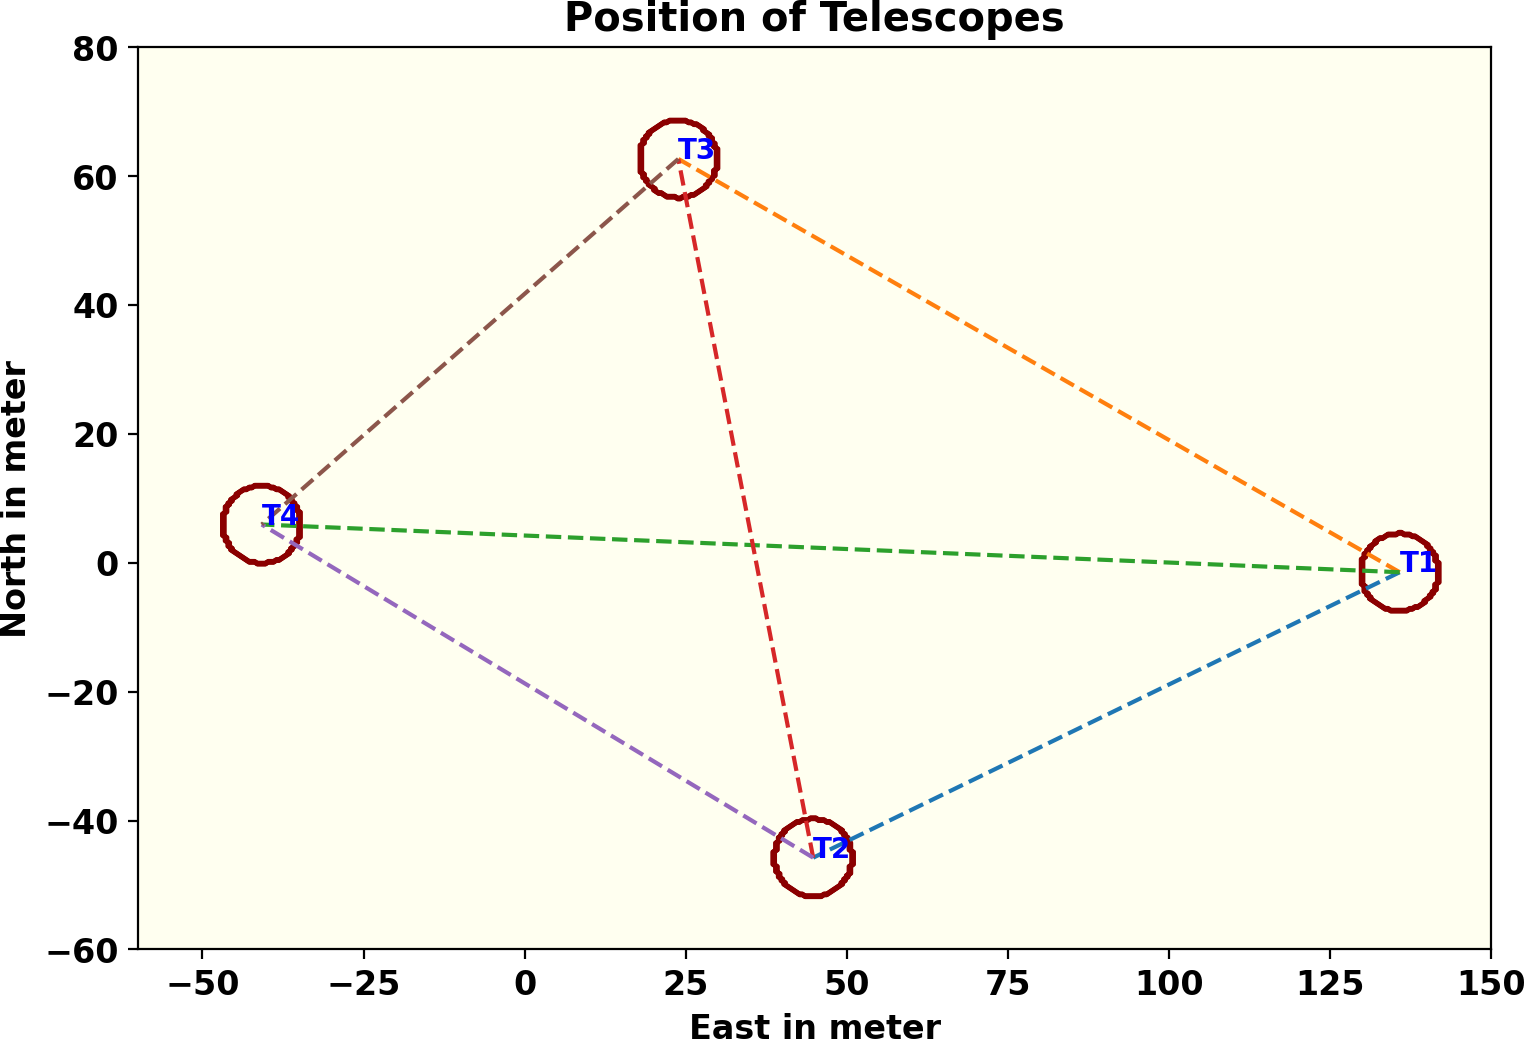
\includegraphics[width=\linewidth]{fig/telescope.png}
	\caption{The telescope configuration with similar properties each used to simulate the signal for II.}
	\label{fig:teles}
\end{figure}
\begin{figure}
	\centering
	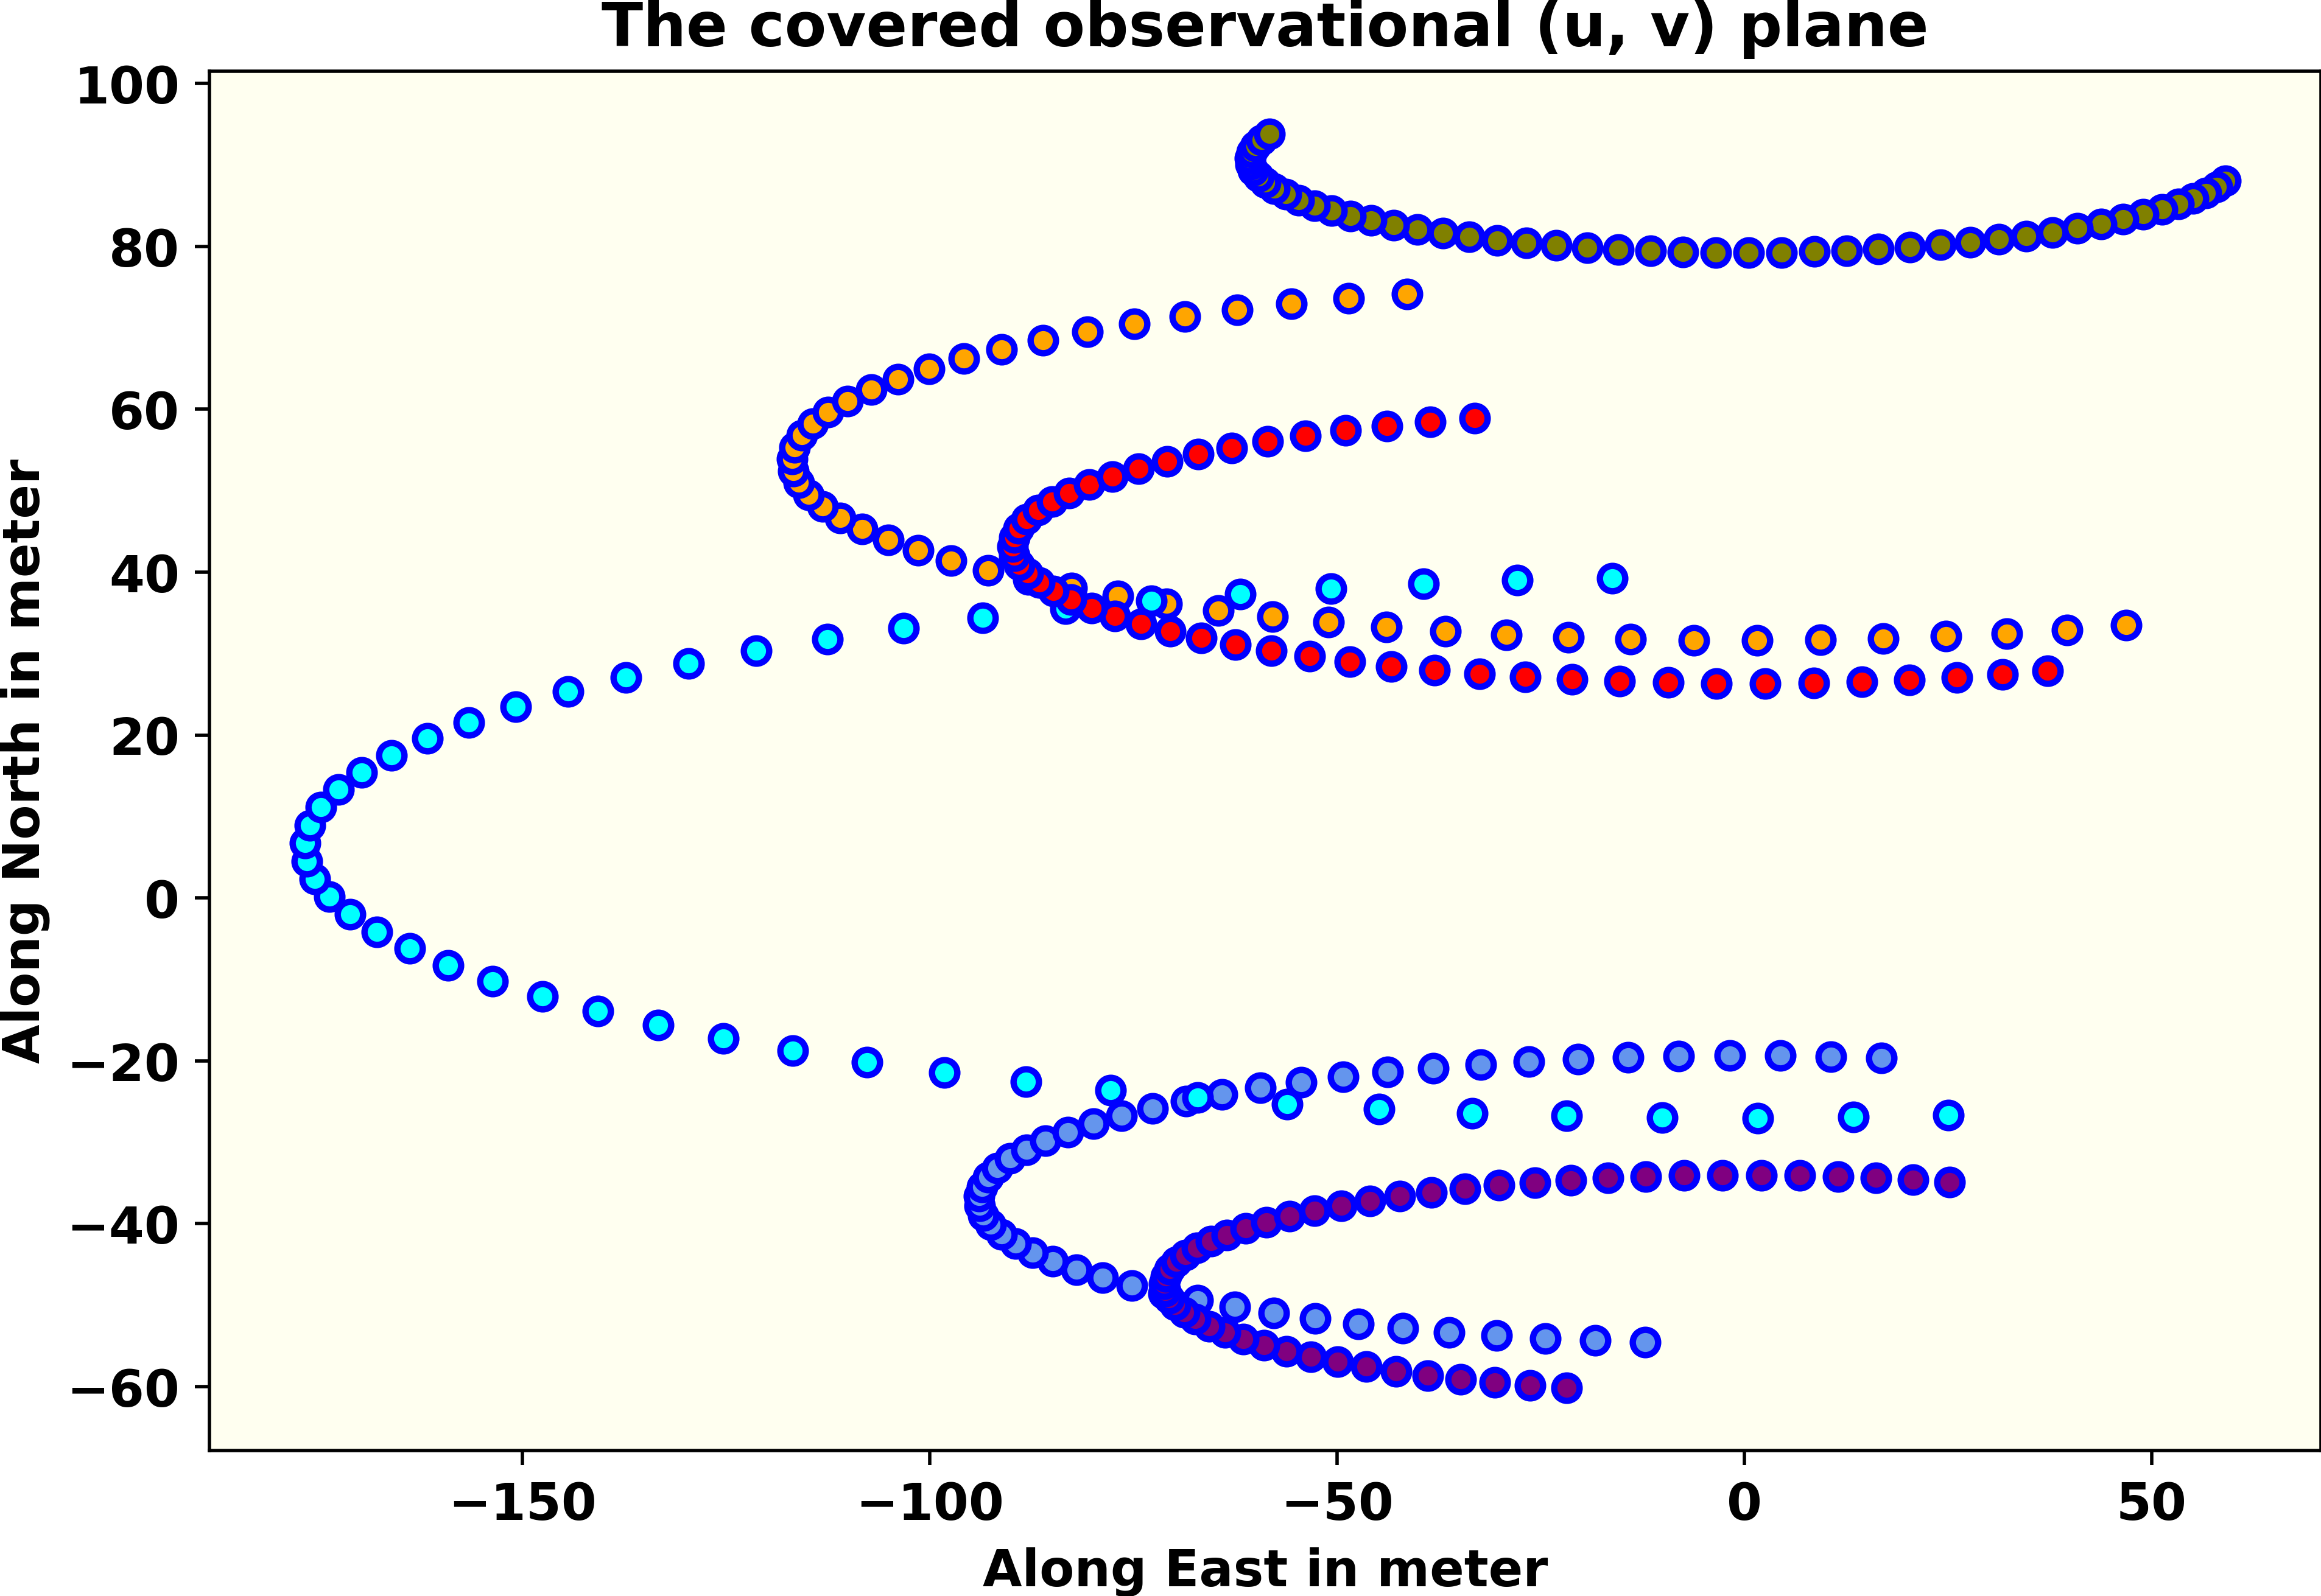
\includegraphics[width=\linewidth]{fig/baseline.png}
	\caption{The tracking of baselines with four telescopes arranged in fig.~\ref{fig:teles} for one night of observation.}
	\label{fig:base}
\end{figure}
\begin{figure}
	\centering
	\includegraphics[width=0.8\linewidth]{fig/ellipse/ellipse6018.jpg}
	\caption{This figure shows the simulated fast rotating star. The brightness is highest at the pole and there is gravitational darkening at the equator.}
	\label{fig:image}
\end{figure}
\begin{figure*}
	\centering
	\begin{subfigure}{0.5\linewidth}
		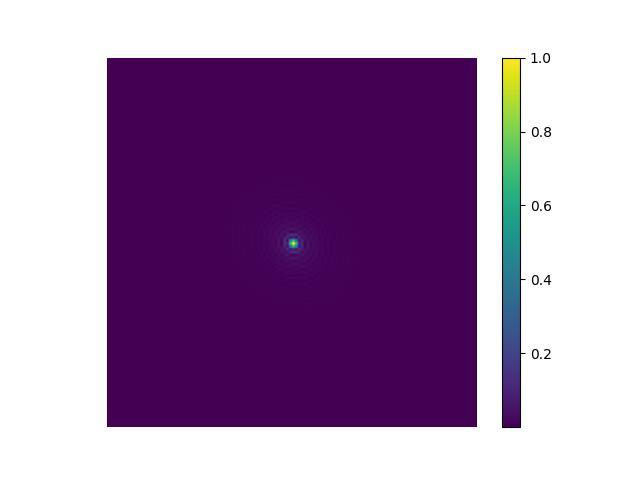
\includegraphics[width=\linewidth]{fig/ft/ft.jpg}
		\caption{The fourier transform of source.}
	\end{subfigure}\hfill
	\begin{subfigure}{0.5\linewidth}
		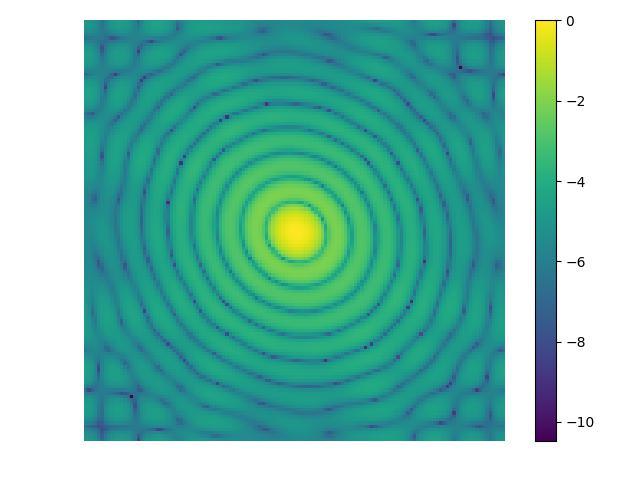
\includegraphics[width=\linewidth]{fig/ft/ft_log.jpg}
		\caption{The logarithmic fourier transform of source.}
	\end{subfigure}
	\caption{Absolute value of the two-dimensional Fast Fourier Transform of fig.~\ref{fig:image} measured by Intensity Interferometry, and observation of maximum (u, v) plane with finite number of baselines can be completed with help of earth's rotation.}
	\label{fig:ft}
\end{figure*}
\begin{figure*}
	\centering
	\begin{subfigure}{0.5\linewidth}
		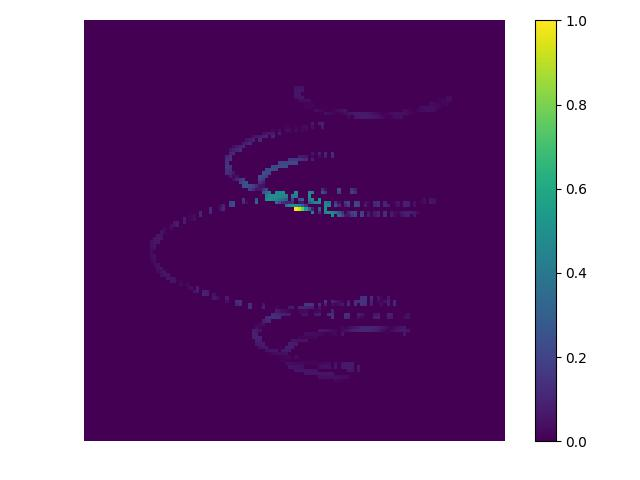
\includegraphics[width=\linewidth]{fig/ft/ft_base.jpg}
		\caption{The fourier transform with baselines.}
	\end{subfigure}\hfill
	\begin{subfigure}{0.5\linewidth}
		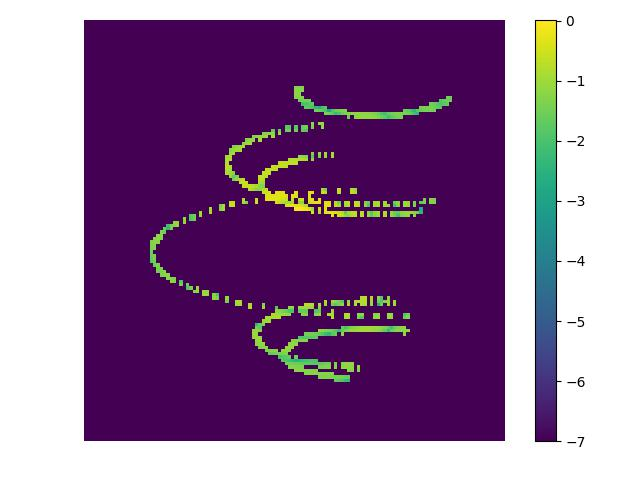
\includegraphics[width=\linewidth]{fig/ft/ft_log_base.jpg}
		\caption{The logarithmic fourier transform with baselines.}
	\end{subfigure}
	\caption{The left panel shows the absolute value of the two-dimensional Fast Fourier Transform of fig.~\ref{fig:image} measured by baselines shown in fig.~\ref{fig:teles}. The right panel shows the same on logarithmic scale}
	\label{fig:ft_base}
\end{figure*}
The primary purpose of IACTs is the study of high energy gamma rays (with energy $E\ \geq 30$ GeV) reaching the Earth from cosmic sources, entering the Earth's atmosphere and seeding the Cherenkov showers in the upper atmosphere due to multiple scattering. These telescopes have an array of mirrors that focus the light onto a set of photo-multiplier tubes (PMTs) \cite{aleksic2016major}. 
\textcolor{blue}{In the simulation model adopted here, a set of four IACTs with similar properties each are considered. The positional configuration of these IACTs is shown in fig.~\ref{fig:teles}. The optical signal guided into a PMT is filtered using a spectral filter with chosen mean observational wavelength $\lambda$ and corresponding bandpass $\Delta \lambda$. 
Use of filters helps in not only reducing back ground noise, but in improving the signal quality and the efficiency of the PMTs also. Filtering background sky light becomes even more significant in II observations as these observations are carried out around full moon nights. Needless to mention that light of the stellar source is focused on the PMT during the II observations.}

The significance of the signal can be expressed as the signal-to-noise ratio (SNR), which depends on many factors. However, most importantly, it does not depend on optical bandwidth $\Delta {\mathrm {\nu}}$ of radiation for two telescope correlation. The explanation of independence of SNR from  $\Delta {\mathrm {\nu}}$ is given in the end of subsection 4.1 of \cite{10.1093/mnras/stab2391}.  
\begin{equation}
	SNR = A \cdot \alpha \cdot q \cdot n \cdot F^{-1} \cdot \sigma \cdot \sqrt{\frac{T \Delta f}{2}} \cdot \abs{V_{12}}^{2}
	\label{eq:SNR}
\end{equation}
here, $A$ is the total mirror area, $\alpha$ the quantum efficiency of the PMTs, $q$ the quantum efficiency of the remaining optics, and $n$ the differential photon flux from the source. The excess noise factor of the PMTs is accounted with $F$, $T$ denotes the observation time, and $\sigma$ is the normalized spectral distribution of the light (including filters) \cite{acciari2020optical}. The signal (S) and noise (N) can be understand using eqns.\ref{eq:signal} and \ref{eq:SNR} as
\begin{equation}
	S = \frac{\Delta f}{\Delta \nu} \abs{V_{12}}^2
\end{equation}
and
\begin{equation}
	N = (A \cdot \alpha \cdot q \cdot n \cdot F \cdot \sigma \cdot \Delta \nu)^{-1}\sqrt{\frac{2 \Delta f}{T}}
\end{equation}
While most of the parameters can be optimized with hardware, the only way to obtain a better SNR is to increase the observation time T with fixed telescopes. 
 
\textcolor{red}{Points to be discussed: 
\begin{itemize}
\item{Should/Can the final expression for SNR in eq.(\ref{eq:SNR}) be written in terms of $\rho(\tau)$ of eq.(\ref{eqn:pearson}) or $c$ (\ref{eq:norm_contrast2}) in stead of $\vert V_{12}\vert^2$?}
\item{It would be better to generalize the eq.(\ref{eq:norm_contrast2}) to include the signals from all the baseline pairs.}
\end{itemize}}
\subsection{Baseline considerations}
The measurement of the size of stellar objects through absolute visibility depends on the distance between the telescopes, which is called the baseline $d$. 
\begin{equation}
	V_{12}(d) = \frac{c(d)}{c(0)}
	\label{eq:angular_size_meas}
\end{equation}
\textcolor{blue}{For achieving a good SNR with a given telescope configuration, the largest possible observational plane that can be covered is always desirable \citep{acciari2020optical, abeysekara2020demonstration}.}
\begin{comment}
{\st{However, this work needs a good SNR value for high precision of measurement, so the large covered observational plane with telescopes is a necessity for II \citep{acciari2020optical, abeysekara2020demonstration}.} }
\end{comment}
If the source is at the zenith, the coordinates in the Fourier plane ($u,v$) are given by:
\begin{equation}
	(u,v) = \frac{1}{\lambda} (d_E, d_N)
\end{equation}
where $d_E$ and $d_N$ are the baselines expressed in north and east coordinates. 
\textcolor{blue}{But not all sources are at the zenith, and the telescopes are stationary and may also have different relative altitudes $d_A$ depending on the available terrain. Therefore, the Earth's rotation needs to be factored in for covering the maximum observational plane through the rotated baselines. 
For a given stellar source with declination $\delta$, hour-angle $h$ observed by telescopes at latitude $l$, equation (\ref{eq:baseline_rot}) provides the rotated
baselines for a given pair of telescopes \citep{dravins2013optical, saha2020theory}
\begin{equation}
\begin{pmatrix} u\\ v\\ w\\ \end{pmatrix} = R_x(\delta) \cdot R_y(h) \cdot R_x(-l) \begin{pmatrix} d_E \\ d_N \\ d_A \\ \end{pmatrix}
	\label{eq:baseline_rot}
\end{equation}
}
%\end{comment}
\begin{comment}
\st{
Equation (\ref{eq:baseline_rot}), which traces an ellipse for every pair of telescopes. Furthermore, the different altitudes $B_A$ of the telescopes must be considered \cite{dravins2013optical, saha2020theory}.  
\begin{equation}
	\begin{pmatrix} u\\ v\\ w\\ \end{pmatrix} = R_x(\delta) \cdot R_y(h) \cdot R_x(-l) \begin{pmatrix} d_N\\ d_E\\ d_A\\ \end{pmatrix}
	\label{eq:baseline_rot}
\end{equation}
here, $\delta$ is the declination and $h$ is the hour angle of the stellar source, and $l$ is the latitude of the telescopes.}
\end{comment}
The three rotation matrices $R_i$ correspond to the fundamental representation of the SO(3) group \cite{saha2020theory}. Fig.~\ref{fig:base} shows the track of six baselines generated from the telescopes (fig.~\ref{fig:teles}) due to Earth's rotation. Since every pair of telescopes traces an ellipse in the Fourier plane, the total number of ellipses scales as follows:
\begin{equation}
	\label{eq:N_telescopes}
	\mathcal{N} = \frac{N_T \cdot (N_T -1)}{2}
\end{equation}
where $N_T$ is the number of telescopes considered.
As the number of baselines increases non-linearly, II benefits greatly from a large number of telescopes. The planned Cherenkov Telescope Array (CTA) will cover the maximum observational plane and provide insight into stellar objects with optical wavelengths in the future.

\subsection{An Object: Fast Rotating Stars}
In our work presented here, we simulate a single fast-rotating star to test image reconstruction using a GAN. Fast rotation causes stars to take on an oblate shape, flattening at the poles and bulging at the equator due to the existence of stronger centrifugal force \cite{von1924radiative, 1999A&A...347..185M}. Fig.~\ref{fig:image} shows one of the simulations of such a fast-rotating star, \st{where the star takes on an elliptical shape} with brightness distributed across its surface. The brightness is at its maximum at the poles and minimum at the equator, a phenomenon known as gravity darkening \cite{lucy1967gravity}. This effect has been observed first through the interferometric and spectroscopic data from the CHARA Array for the fast-rotating star Regulus \cite{mcalister2005first}. Fast-rotating stars are crucial for understanding various astrophysical processes, including stellar evolution, structure, and \textcolor{red}{dynamics(??? Can we be more elaborate here?)} over time.

Intensity Interferometry measures/counts photons arriving at the telescopes from the stellar object. The correlation of these photon arrivals at the telescopes results in squared visibility (explained in subsection.\ref{sec:signal}). According to Van Cittert Zernike's theorem, this signal is the Fourier transform of brightness distribution in the sky. Fig.~\ref {fig:ft} shows represents the Fourier Transform of the source shown in fig.~\ref{fig:image} using II on linear and logarithmic scale. 
\sout
{However, we do not have an existing technique to observe the complete signals, and we could capture some parts of it only with a one-night simulation, which has been shown in fig.~\ref{fig:ft_base}. It is the covered observational plane using the baselines shown in fig.~\ref{fig:teles}. However, the upcoming CTA promises to cover the maximum observational plane for stellar objects.}
\textcolor{blue}{In order to observe a real stellar source in the sky, however, we would need to receive photons from each point on the surface of the source. This would require infinite number of baselines observing the source over a long enough duration. This demand is obviously not feasible. We have finite number of baselines corresponding to the finite number $N_T$ of telescopes at our disposal and finitely budgeted observation schedule. Therefore, as a pilot, what we have attempted in this work is to simulate the II observation of a sky source over one night duration. Using this finite amount of signal of one night's observation, we have attempted to train a Generative Adversarial Network (GAN) to construct the image of the source.}  

\textcolor{red}{My comments: Suppose we do more simulations with say 8 and 16 telescopes covering the effective ground area, but obviously with 28 and 120 baselines respectively. We can then, perhaps, evolve/suggest some kind of measure (or scale) of quality in resultant image reconstruction with number of telescopes. May be some form of ratios of the SNRs would provide a good comparison. {\bf How much more computationally expensive would it become?}}
\section{Generative Adversarial Networks}

Generative Adversarial Networks (GANs) were introduced by \cite{goodfellow2014generative}. The underlying concept is straightforward: it involves two competing networks. The first network, known as the Generator, produces new images based on an input image. These will be referred to as generated images. The second network, the Discriminator, attempts to distinguish between the generated image (predicted image) and the real image (ground truth) using Discriminator loss function.

Through the alternating training of these networks, the generated images gradually become indistinguishable from the real images. Essentially, this process constitutes a two-player min-max game --- a classic problem in game theory. The original formulation of GANs is given by:
\begin{equation}
	\centering
	\begin{aligned}
		\min_{G} \max_{D} V(D, G) &= \mathbb{E}_{x \sim p_{\rm data}(x)} \left[ \log D(x) \right] \\
		&+ \mathbb{E}_{z \sim p_{z}(z)} \left[ \log \left( 1-D(G(z)) \right) \right]
	\end{aligned}
	\label{eq:Basic_GAN}
\end{equation}
where $V(D, G)$ denotes the value function of the min-max game.

The objective is to learn the Generator's distribution, \(p_G\), over the data \(x\). We begin with input noise variables \(p_z(z)\) and employ two perceptrons, \(G(z; \theta_G)\) and \(D(x; \theta_D)\), parameterized by \(\theta_i\) with \(i = G \ \mathrm{or}\ D\) respectively. Here, \(G(z)\) is a differentiable function that maps \(z\) to the data space \(x\), while \(D(x)\) represents the probability that \(x\) originates from real data. The problem can be reformulated as:
\begin{equation}
	\centering
	\begin{aligned}
		\max_{D} V(G, D) &= \mathbb{E}_{x \sim p_{\rm data}} \left[ \log D^{*}_{G}(x) \right] \\ 
		&+ \mathbb{E}_{x \sim p_{G}} \left[ \log \left( 1 - D^{*}_{G}(x) \right) \right]
	\end{aligned}
	\label{eq:GAN_reformulated}
\end{equation}
where \(D^{*}_{G}\) denotes the optimum of the discriminator for a given fixed generator, as shown in equation (\ref{eq:Disc_optimum}). It can be demonstrated that the global optimum of equation (\ref{eq:GAN_reformulated}) is achieved if and only if \(p_G = p_{\rm data}\). Furthermore, if both \(G\) and \(D\) are allowed to reach their respective optima, then \(p_G\) converges to \(p_{\rm data}\). A more comprehensive discussion of the problem, including proofs, is provided in \cite{goodfellow2014generative}.
\begin{equation}
	\centering
	D^*_G(x) = \frac{p_{\rm data}(x)}{p_{\rm data}(x) + p_G(g)}
	\label{eq:Disc_optimum}
\end{equation}

Subsequently, the GAN framework was extended to a conditional model \citep{mirza2014conditional}. In this formulation, both the Generator and the Discriminator receive additional information $y$, and the value function of the conditional GAN (cGAN) is expressed as:
\begin{equation}
	\centering
	\begin{aligned}
		V(D, G) &= \mathbb{E}_{x \sim p_{\rm data}(x)} \left[ \log D(x|y) \right] \\
		&+ \mathbb{E}_{z \sim p_{z}(z)} \left[ \log \left( 1-D(G(z|y) \right) \right]
	\end{aligned}
	\label{eq:conditional_GAN}
\end{equation}
\cite{isola2017image} further observed that combining the cGAN from Eq.~\eqref{eq:conditional_GAN} with the traditional L1 loss improves the results, as the Generator is encouraged to produce outputs closer to the ground truth. Hence, the function that is minimized is:
\begin{equation}
	\centering
	L_{tot} = \arg \min_{G} \max_{D} V(D, G) + \lambda \cdot L_1(G)
	\label{eq:total_gen_loss}
\end{equation}
with the choice $\lambda = 100$ and
\begin{equation}
	\centering
	L_1(G) = \mathbb{E}_{x,y,z} \left[ ||{y - G(x,z)}||_1 \right]
	\label{eq:l1_loss}
\end{equation}
This type of network has demonstrated remarkable robustness across a variety of applications. For example, it can generate colored images from grayscale inputs based on architectural labels, transform images from day to night, and even predict maps from satellite data. A more extensive list of applications is provided in \cite{isola2017image}.


\subsection{Generator}
As discussed above, in a GAN the Generator is responsible for producing synthetic data—in this case, images that resemble those of a fast-rotating star. In this work, the Generator is implemented as a U-Net convolutional network \citep{ronneberger2015u}. In such architectures, the image's spatial resolution is first reduced through downsampling and then restored via upsampling, resulting in a U-shaped structure. The downsampling process typically involves convolutional layers followed by a strided operation (with a stride of 2) to effectively subsample the image, and a leaky version of the Rectified Linear Unit (LeakyReLU) is employed as the activation function.

In contrast, the upsampling process uses only the standard Rectified Linear Unit (ReLU) for neuron activation. This stage also comprises convolutional layers followed by operations with a stride of 2 to upscale the image to a higher resolution. Additionally, a dropout layer is introduced at the beginning of the upsampling phase to mitigate overfitting of the Generator model \citep{isola2017image}.

After generating images, the Generator aims to deceive the Discriminator into classifying the generated images as real. The extent to which the Generator succeeds in this deception is quantified by the GAN loss. When the Discriminator is unable to distinguish between the generated and real images (i.e., when the GAN loss is minimized), the Generator is considered to have reached an optimal state. Conversely, if the generated image fails to fool the Discriminator, the Generator produces a new image for further comparison with the real image. Additionally, the Generator's performance is evaluated using another metric known as the L1 loss, which is defined as the mean absolute error between the pixels of the real image and those of the generated image. Balancing the minimization of both the GAN loss and the L1 loss enables the Generator to produce images that are not only realistic but also faithful to the input data. 

\subsection{Discriminator}
The Discriminator is tasked with classifying the images produced by the Generator as either real or fake. It takes a real image from the dataset (often referred to as the target image for the Generator) and provides feedback to guide the Generator toward producing more accurate images. In this work, the PatchGAN model \citep{isola2017image} is employed as the Discriminator. Unlike a traditional global classifier, PatchGAN evaluates individual patches of the image, outputting a grid of predictions rather than a single scalar value.

The Discriminator’s architecture begins with an initializer that accepts both the input (generated) images and the corresponding real images. Initially, Salt-and-Pepper noise is added to the input images. PatchGAN then reduces the spatial dimensions of the images to extract localized features, ensuring the model focuses on smaller regions. In this downsampling stage, a leaky version of the Rectified Linear Unit (LeakyReLU) is applied in the convolutional layers, similar to the approach used in the Generator.

Subsequently, zero padding is applied—adding rows and columns of zeros around the images—to prevent the loss of spatial information during convolution and to facilitate the extraction of deeper features from the downsampled output. Following this, batch normalization is employed to stabilize learning by normalizing activations, and the Discriminator begins classifying each patch as real or fake. This is followed by additional layers involving LeakyReLU activation, zero padding, and convolution, culminating in a final prediction that the Generator uses as feedback.

The effectiveness of the Discriminator is measured by its ability to distinguish between real and fake images, quantified through the Discriminator loss. This loss is composed of two parts: one that measures how accurately the Discriminator identifies real images (by comparing predictions to a target value of 1) and another that assesses how accurately it identifies fake images (by comparing predictions to a target value of 0). Together, these loss components ensure that the Discriminator improves its classification performance, which in turn challenges the Generator to produce increasingly realistic images.

\section{Network Parameters}
\begin{figure*}
	\vspace{-1cm}
	\centering
	%\begin{subfigure}{\linewidth}
	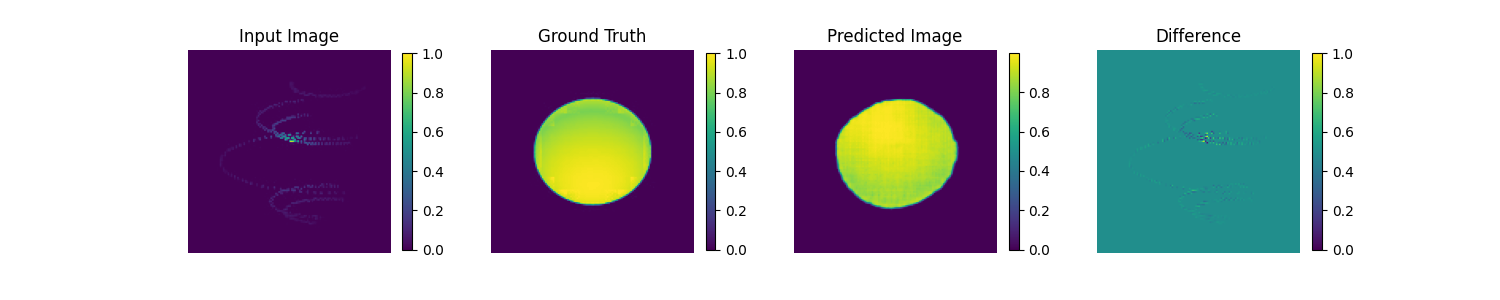
\includegraphics[width=\linewidth]{fig/testing_image/image_0.png}
	%\end{subfigure}
	%\begin{subfigure}{\linewidth}
	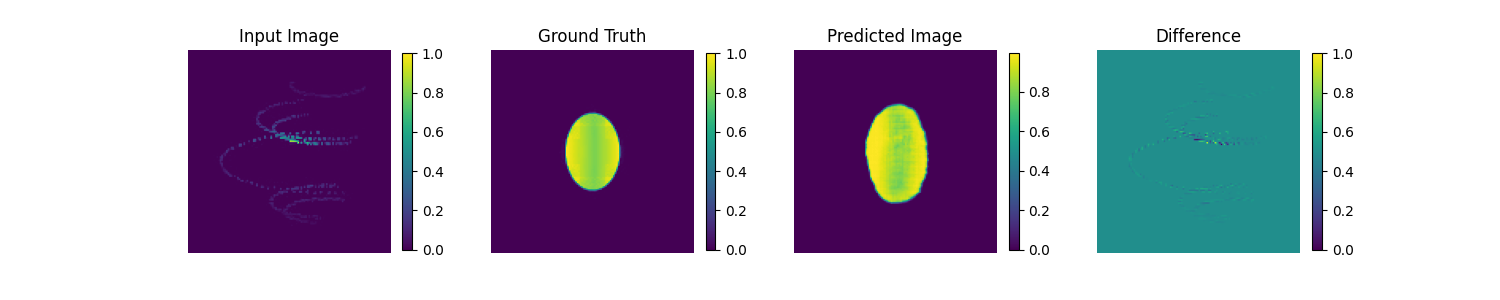
\includegraphics[width=\linewidth]{fig/testing_image/image_16.png}
	%\end{subfigure}
	%\begin{subfigure}{\linewidth}
	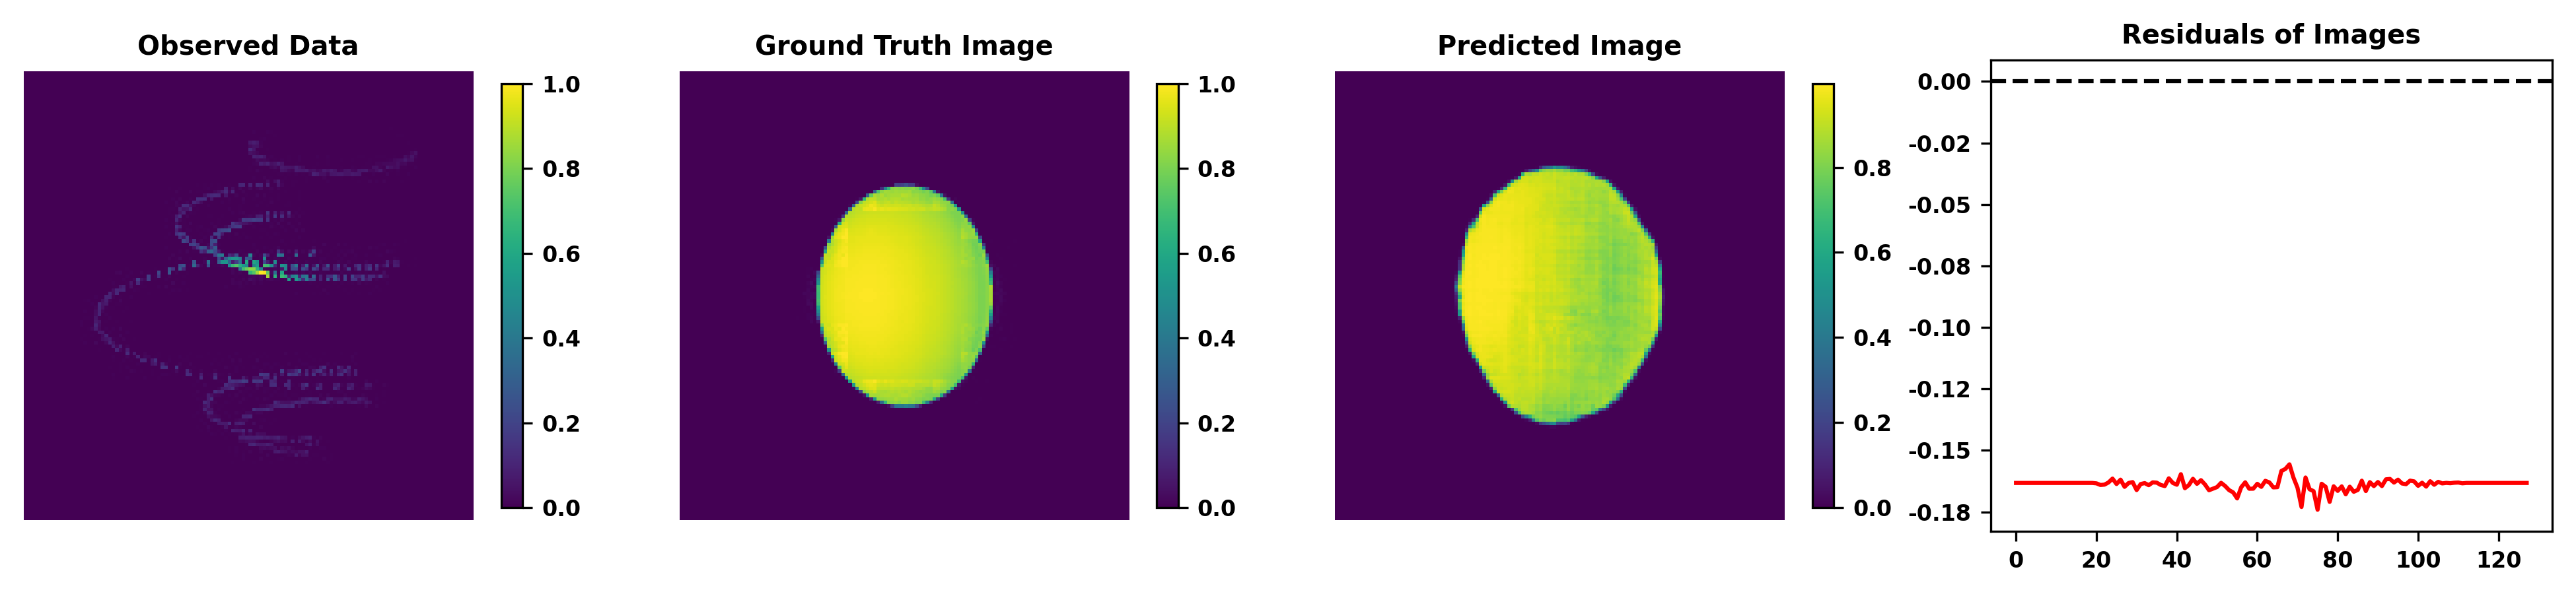
\includegraphics[width=\linewidth]{fig/testing_image/image_35.png}
	%\end{subfigure}
	%\begin{subfigure}{\linewidth}
	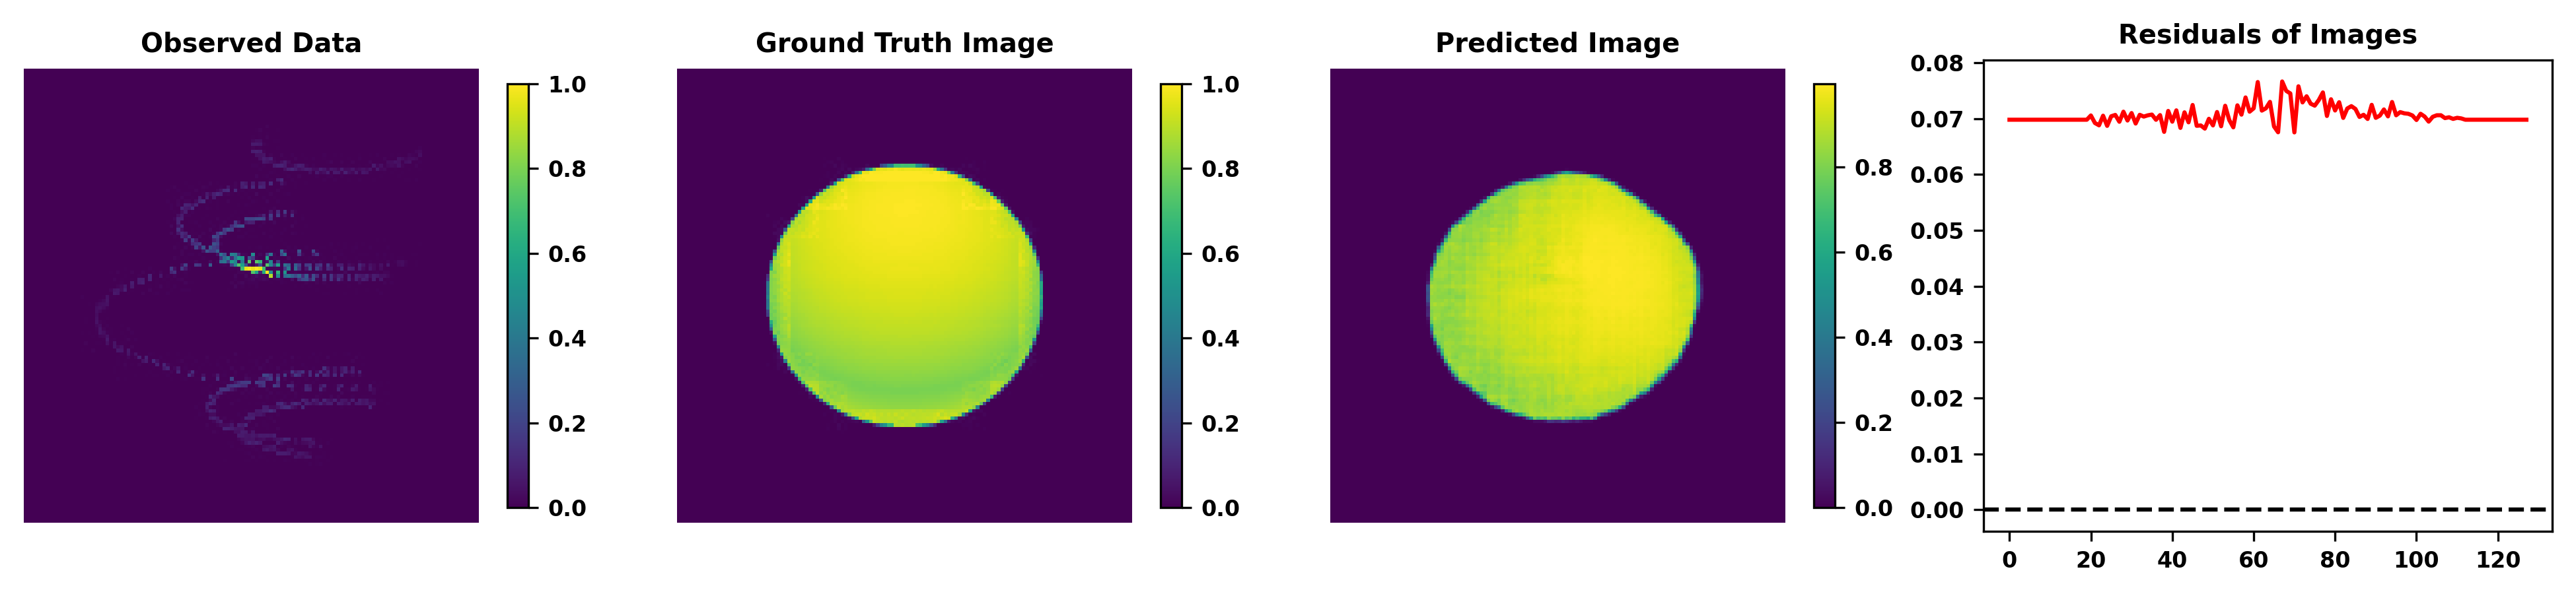
\includegraphics[width=\linewidth]{fig/testing_image/image_38.png}
	%\end{subfigure}
	%\begin{subfigure}{\linewidth}
	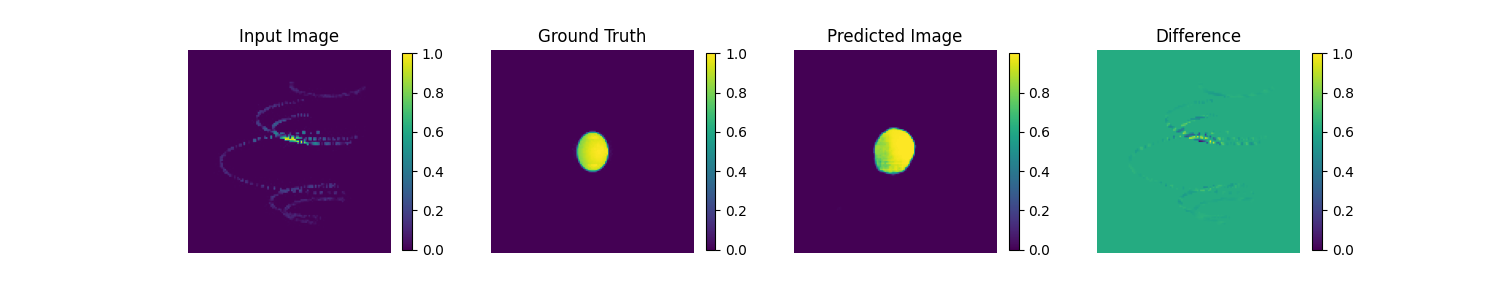
\includegraphics[width=\linewidth]{fig/testing_image/image_42.png}
	%\end{subfigure}
	%\begin{subfigure}{\linewidth}
	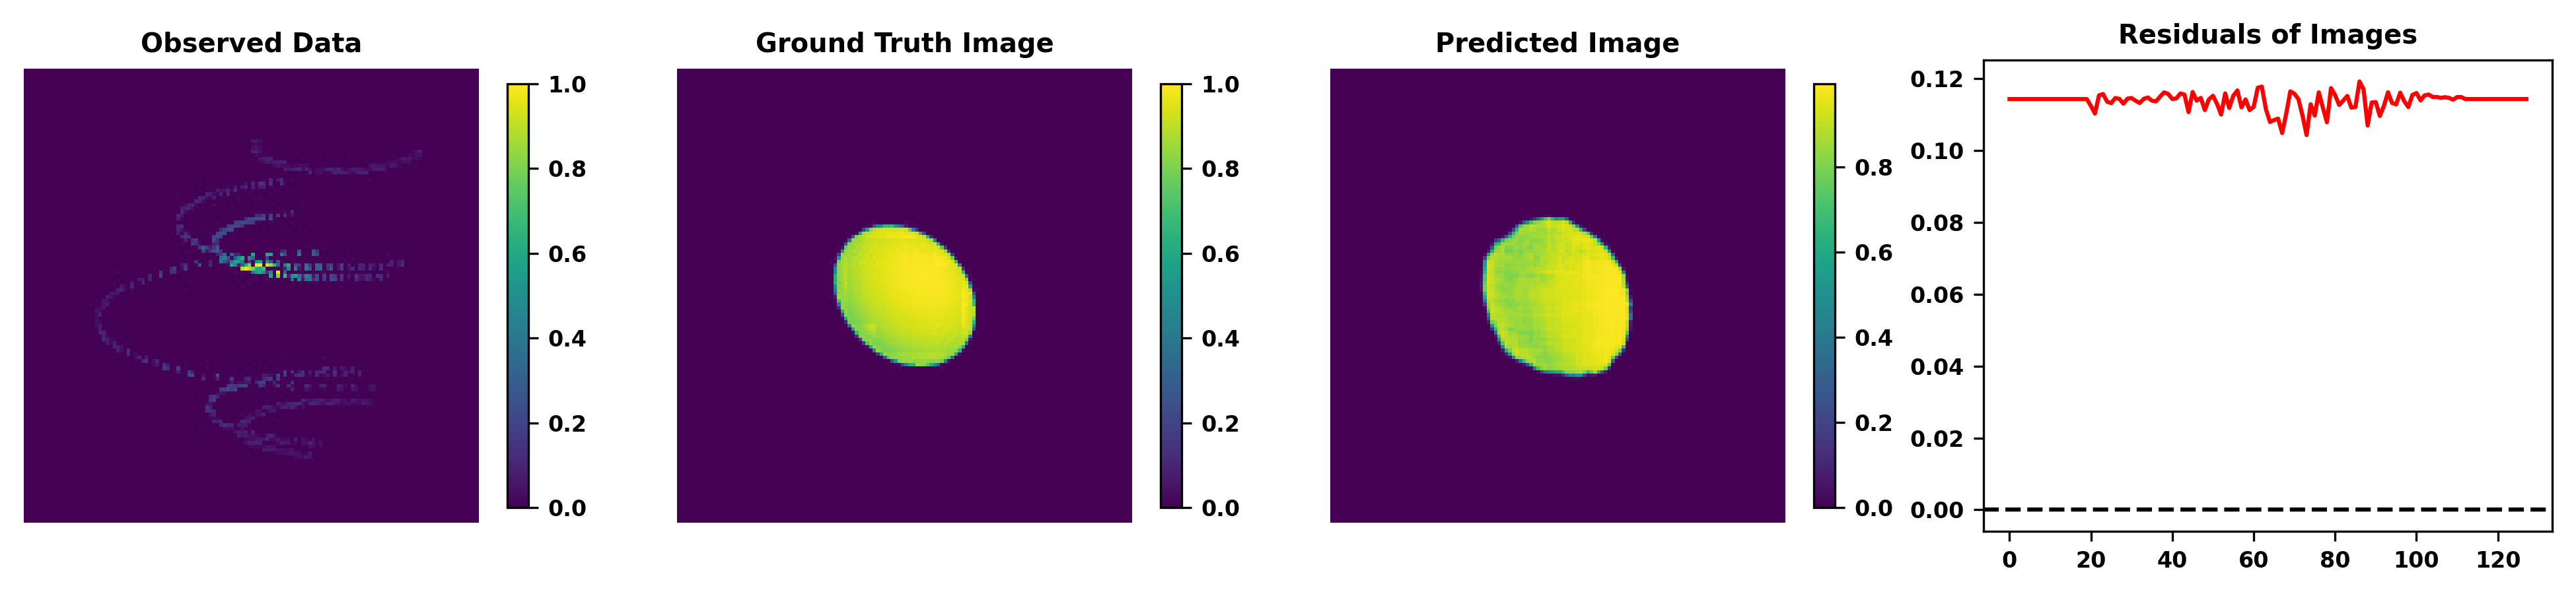
\includegraphics[width=\linewidth]{fig/testing_image/image_47.png}
	%\end{subfigure}
\caption{Examples results of GAN for II. The left panels are signals using six baselines, which work as input for GAN. The first middle panel is the real image, also called ground truth, and GAN tries to mimic it during the training. The second middle panel is the reconstructed image, also called the predicted image, with trained GAN, and the end panel is the difference between the ground truth and the predicted image.}
	\label{fig:GAN}
\end{figure*}
Here, we discuss the parameters of the GAN architecture used for reconstructing images of stellar objects using II. Given the adversarial nature of GANs—where the Generator and Discriminator engage in a min-max game—careful tuning of key parameters is critical to ensure that both networks are well-balanced for effective training.

\begin{figure*}
  %\begin{subfigure}{0.33\linewidth}
  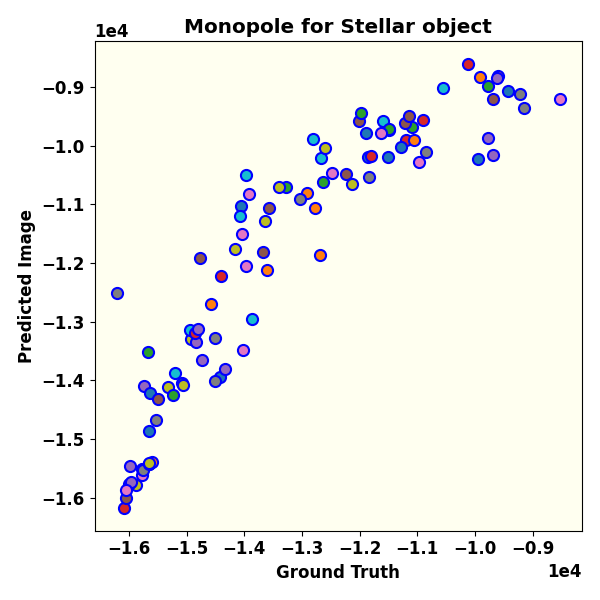
\includegraphics[width=.32\linewidth]{fig/moments/mom0.png}\hfil
  %\caption{The monopole.}
  %\label{fig:mom1}
  %\end{subfigure}\hfill
  %\begin{subfigure}{0.33\linewidth}
  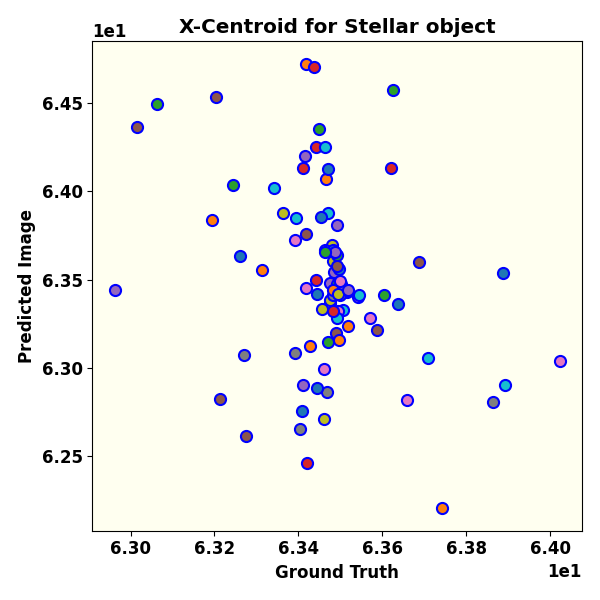
\includegraphics[width=.32\linewidth]{fig/moments/mom1.png}\hfil
  %\caption{The centroids along x direction.}
  %\label{fig:mom2}
  %\end{subfigure}\hfill
  %\begin{subfigure}{0.33\linewidth}
  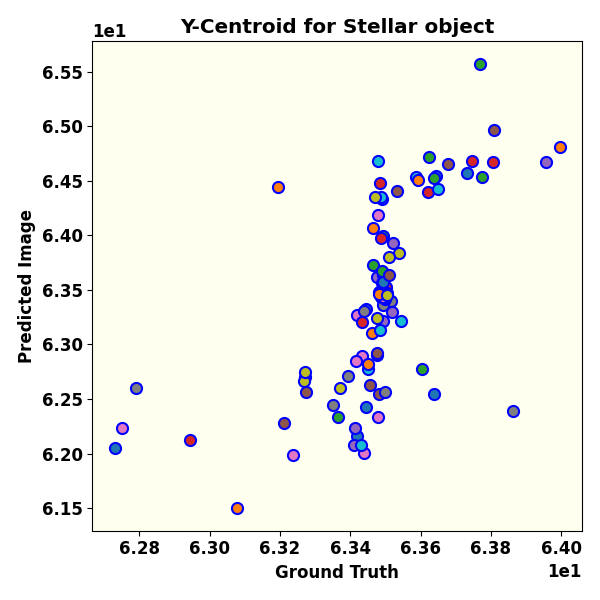
\includegraphics[width=.32\linewidth]{fig/moments/mom2.png}
  %\caption{The centroids along y direction.}
  %\label{fig:mom3}
  %\end{subfigure}\hfill
  \caption{This set of figures shows the comparison of monopole, x-centroid, and y-centroid for ground truth and predicted images generated by trained GAN.}
	\label{fig:cen}
\end{figure*}
\subsection{Data Preparation}
First, we simulate fast-rotating stars, modeling them as oblate spheroids with varying radii and an oblateness ranging between 0.5 and 1. We also consider different viewing angles, assuming a linear dependence for the effect of gravity darkening. The traced ellipses result from integrating over the source's hour angle. For hyperparameter tuning and comparing different telescopes, the total observing duration is set to approximately 11.5 hours. Finally, the ellipses are plotted, converted into grayscale images, resized, and stored as raw arrays to facilitate further analysis.

First, Salt and Pepper noise is introduced at a rate of \(\alpha\) (usually 0.5\%). Then, the images are resized and their mean is subtracted. A two-dimensional Fast Fourier Transform, along with a Fourier shift, is applied, yielding a complex number for each pixel. Since II does not measure phase, the absolute value is calculated (as shown in Fig.~\ref{fig:ft} on both linear and logarithmic scales for visualization). 

Next, sparse sampling is introduced via pixel-wise multiplication between the absolute-valued Fourier-transformed image (Fig.~\ref{fig:ft}) and the sparse sampling map (Fig.~\ref{fig:base}). The result is a map in the Fourier plane featuring several ellipses, which is also referred to as the sparse sampling map (Fig.~\ref{fig:ft_base}). This map represents the sparse sampling for Fig.~\ref{fig:image}, corresponding to the source observed with four telescopes (Fig.~\ref{fig:teles}). 

Finally, the pixels are normalized and converted to 8-bit integers. This image represents the sparsely sampled phaseless visibility as it can be measured with II. The image shown in Fig.~\ref{fig:ft_base} serves as the input for the GAN, which also requires the corresponding ground truth image. Consequently, the simulated stars are resized using the same algorithm and converted to 8-bit integers to reduce bias. The GAN must have access to the ground truth corresponding to each input image; therefore, the input and ground truth images are merged side-by-side (as shown in Fig.~\ref{fig:GANinput}) and used to train the GAN. This procedure is applied to all simulated stars, with 10\% used as test data, 10\% as validation data, and the remaining 80\% as training data.


\subsection{GAN Architecture}
The GAN used in this work is based on pix2pix, which utilizes a conditional GAN (cGAN) as discussed in the previous section \citep{isola2017image}. This architecture is highly robust and has already been applied to various problems. For instance, the TensorFlow tutorials\footnote{\url{https://www.tensorflow.org/tutorials/generative/pix2pix}} demonstrate its application to a dataset of architectural facades. However, to adapt the pix2pix GAN for the phase retrieval problem, some modifications are necessary. The network is implemented using the TensorFlow library \citep{abadi2016tensorflow}, calculations are performed with scipy \citep{virtanen2020scipy}, and plots are generated with matplotlib \citep{4160265}.

\subsection{Hyperparameter Tuning}
The GAN used in this work depends on several parameters, which are explained briefly below \citep[for a more in-depth discussion, see][]{murphy2022probabilistic}.

The learning rate of the optimizer determines how much the model updates its parameters with each iteration. A learning rate that is too small may lead to underfitting, while one that is too large can render the model unstable. Therefore, selecting an appropriate learning rate is crucial \citep{murphy2022probabilistic}. Fig.~\ref{fig:Plot_learning_rate_loss} illustrates the effect of different learning rates on both the Generator and Discriminator losses. As expected, lower learning rates result in fewer outliers in the loss functions, indicating more stable updates. Although all models eventually stabilize at a similar level, lower learning rates are preferred.

The kernel size refers to the dimensions of the convolutional kernel used in the network, determining how many pixels are combined to produce a new pixel. A larger kernel size can capture features spanning several pixels, but it may also incorporate unrelated features. As shown in Fig.~\ref{fig:Plot_kernel_size_loss}, the kernel size does not have a significant impact on the loss functions; however, smaller kernel sizes tend to produce more outliers, suggesting that either the Generator or Discriminator may gain an advantage. Therefore, a kernel size of 5 is preferred.

The amount of noise is controlled by two parameters, \(\alpha\) and \(\beta\), which indicate the percentage of pixels altered to either black or white—hence the term Salt and Pepper noise. Here, \(\alpha\) is applied to the real image, while \(\beta\) is applied to the generated image. Different ratios \(\frac{\alpha}{\beta}\) can lead to varying model performance; however, our results indicate that distinct noise rates do not significantly affect the loss functions. Figure~\ref{fig:Plot_noise_loss} shows the loss functions for smaller images ($64 \times 64$), and due to the negligible impact, this analysis was not repeated for larger images.

The batch size defines the number of images processed simultaneously by the network. Smaller batch sizes have been observed to improve generalization \citep{prince2023understanding}. As illustrated in Fig.~\ref{fig:Plot_batchsize_loss}, processing two images at once results in fewer outliers. However, because a larger batch size significantly increases training time, a batch size of 1 is used.

When training GANs, one strategy to potentially boost performance is to give the Discriminator an advantage by increasing its number of training steps before returning to the Generator's training. While this can lower the Discriminator loss—as shown in Fig.~\ref{fig:Plot_discrep_loss}—it also increases training time and leads to a slight rise in the Generator loss. Since the generated images do not noticeably improve with additional Discriminator training, both networks are typically trained with the same number of steps.

Finally, the degree of sparse sampling can be varied to provide the model with access to more pixels. Increasing the number of telescopes results in more baselines and, consequently, more available pixels. Fig.~\ref{fig:Plot_telescopes_loss} shows the loss functions for different numbers of telescopes. There is a significant disparity in performance, partly because the relationship between telescopes and baselines is not linear. For example, the Fourier plane can be sampled along six tracks when using four telescopes, as compared to only one tracks if using only two telescopes. In the case of two telescopes, both the Generator and Discriminator exhibit less smooth training, as indicated by the outliers. Performance improves with three telescopes and becomes very promising with four. Overall, the degree of sparse sampling appears to have the most pronounced effect of all the hyperparameters.

\section{The Reconstructed Image with GAN}
In this section, we will first discuss phase retrieval using hyperparameters, as mentioned earlier, followed by an analysis where multiple sources are trained simultaneously. The best performance for image reconstruction has been observed with a learning rate of $2 \cdot 10^{-4}$, a kernel size of 5x5, and equal noise percentages in original and generated images. The batch size selected is 1, and the Discriminator-Generator receives equal training.

\subsection{The Predicted Image with Trained GAN}
The success of the GAN in training the model for Intensity Interferometry to reconstruct images of fast-rotating stars is demonstrated in Fig.~\ref{fig:GAN}. The GAN was trained on training datasets for 60,000 steps. After training, the GAN was tested on different validation datasets, producing predicted images of a fast-rotating star. Fig.~\ref{fig:GAN} presents a set of four combined images demonstrating the GAN's performance in reconstructing the shape, size, and brightness distribution of the fast-rotating star using II. The left panel shows the signals covered by six baselines, which serve as the input for the Generator to train the GAN. The first middle panel displays the real image, or ground truth, which the Discriminator uses to differentiate between real and generated images from the Generator. During training, the GAN aims to mimic these ground truth images. The second middle panel depicts the reconstructed image, or predicted image, produced by the trained GAN. This panel illustrates the success of the GAN in image reconstruction using II. The right panel shows the difference between the ground truth and the predicted image. This difference should be minimized for high-precision image reconstruction with the application of GAN on II. The predicted images of Fig.~\ref{fig:GAN} showed positive results. It accurately provides visual information about the source's size, shape, and brightness distribution over the surface. It is achieved here using only six baselines. However, the results can be further improved by increasing the number of telescopes to cover maximum (u, v) planes, making the existing and upcoming Cherenkov Telescope Array Observatory (CTAO) an ideal candidate. 

\subsection{Evaluation of GAN using Moments}
The reconstructed images are good enough visually to claim the success of GAN in reconstructing the image using II. However, there is a need for statistical evaluation of this predicted image to guarantee success. So, we use image moments as a statistical method. Image moments are statistical properties that provide information about the reconstructed shape, size, and intensity distribution of the objects in the image. These moments help to quantify key features like the position, orientation, and distribution of brightness in the image, allowing for an objective evaluation of how well the predicted image corresponds to the actual object. We will analyze the consistency and accuracy of the GAN-generated image by comparing its moments to those of the ground truth. It provides a reliable framework for evaluating reconstruction quality, as image moments highlight the subtle differences in geometric and intensity properties that might not be visually apparent. 

The raw moment $M_{ij}$ of an image I(x, y) is defined as \citep{hu1962visual}
\begin{equation}
	M_{ij} = \sum_{x} \sum_{y} x^i y^j I(x, y).
	\label{eqn:Mom}
\end{equation}

The zeroth order raw moment called the monopole is the total intensity of an image. It sums up all the pixel values across the image, providing an overall intensity value. So, the study of monopole provides the total flux of fast-rotating stars here. According to eqn.~\ref{eqn:Mom}, the monopole of an image is calculated as 
\begin{equation}
	M_{00} = \sum_{x} \sum_{y} I(x, y).
\end{equation}
Fig.~\ref{fig:mom1} shows the monopole for 50 different reconstructed images. It shows the linear behavior for the monopole between the ground truth (the real image) along the x-axis and the predicted image (reconstructed image) along the y-axis, which is obvious for different shape-size sources. This result explains the similarity between the total intensity of both images. It ensures that the predicted image has the approximately correct total brightness (the flux) compared to the ground truth. However, monopole does not explain the position, shape, size, and brightness distribution of fast-rotating stars; there is a need for higher-order moments.

The center of mass for the fast-rotating star or any other stellar object is calculated using the centroid (x-centroid and y-centroid). It represents the spatial position of the image and is calculated using first-order raw moment and monopole. The formulation of centroid along the x and y directions is
\begin{equation}
	\begin{aligned}
		&m_x = \frac{\sum_{x} x I(x,y)}{\sum_{x} \sum_{y} I(x, y)} = \frac{M_{10}}{M_{00}} \\
		&m_y = \frac{\sum_{y} y I(x,y)}{\sum_{x} \sum_{y} I(x, y)} = \frac{M_{01}}{M_{00}}
	\end{aligned}  
\end{equation}
Fig.~\ref{fig:mom2} and Fig.~\ref{fig:mom3} show the comparison of the x-centroid and y-centroid for 50 predicted images with respect to ground truths, respectively. The clustering of centroids in a given scale range for all the results explains that the reconstructed image correctly represents the spatial location of the fast-rotating star compared with the ground truth.

Further, these calculated centroids will help to study the shape, size, and brightness distribution of fast-rotating stars in terms of higher-order image moments. For that, the central moment of an image is calculated according to
\begin{equation}
	\mu_{pq} = \frac{1}{M_{00}}\sum_{x} \sum_{y} (x - m_x)^p (y - m_y)^q I(x, y).
\end{equation}
The sum of $p$ and $q$ defines the order of the central moment.

The second order central moment ($\mu_{11}, \mu_{20}, \mu_{02}$) has been shown in Fig.~\ref{fig:struc}, which is used to study the structure of a fast-rotating star along the line of sight of observation (explain in upcoming subsection). All these three plots explain the linear relation of second-order moments again as for monopole and show the success of the application of GAN to reconstruct the image with II.

The information on brightness distribution is gathered using the skewness of the image by calculating third-order central moment ($\mu_{30}, \mu_{03}, \mu_{21}, \mu_{12}$) of images. Fig.~\ref{fig:moments} shows all third-order moments for the ground truth and reconstructed image. The skewness along the x and y axis ($\mu_{30}, \mu_{03}$) to test the GAN for II are acceptable, which can be seen in Fig.~\ref{fig:mom7} and Fig.~\ref{fig:mom8}, where a linear relation exists between ground truth and predicted image. However, the remaining higher moments $(\mu_{21}, \mu_{12})$ shown in Fig.~\ref{fig:mom9} and Fig.~\ref{fig:mom10} are not in good terms specially $\mu_{12}$. Further improvement is possible and needs to be studied.

\subsection{The reconstructed Parameters for object}
The centroids $(m_x, m_y)$ represent the center of the fast-rotating star and spatial location on the image only. However, the calculated second-order central moment defines the orientation, semi-major axis, and eccentricity with respect to the center of the source \citep{teague1980image}. These parameters based on the moments fully describe the two-dimensional ellipse that fits the image data. 

The orientation of a fast-rotating star along the line of sight is defined in terms of second-order central moments as
\begin{equation}
	\theta = \frac{1}{2}\arctan \big(\frac{2\mu_{11}}{\mu_{20} - \mu_{02}}\big).
	\label{eqn:orn}
\end{equation}
The semi-major and semi-minor axis of the stellar object will be calculated with the help of second-order central moment again and denoted as a and b here, respectively
\begin{equation}
	\begin{aligned}
		&a = 2\sqrt{mp + \delta} \\
		&b = 2\sqrt{mp - \delta}
	\end{aligned}
	\label{eqn:semi}
\end{equation}
where,
\begin{equation}
	mp = \frac{\mu_{20} + \mu_{02}}{2}
	\label{eqn:mp}
\end{equation}
and
\begin{equation}
	\delta = \frac{\sqrt{4\mu_{11}^2 + (\mu_{20} - \mu_{02})^2}}{2}.	
	\label{eqn:delta}
\end{equation}
With the help of the axis value, the eccentricity of the fast-rotating star is calculated as
\begin{equation}
	e = \sqrt{1 - a/b}.
	\label{eqn:eccen}
\end{equation}
Eqns.~\ref{eqn:orn}-\ref{eqn:eccen} depending on values explains the elliptical nature of the stellar object (here, fast-rotating star) and provides information on shape and size. However, the information about the brightness distribution is gathered using skewness, which can be understood using third and higher-order moments.

\section{Conclusion}
The challenge of phase retrieval in Intensity Interferometry (II) has been effectively addressed through the application of machine learning techniques, particularly with Generative Adversarial Networks (GANs). Our study demonstrates that using a GAN on II data successfully recovers the size, shape, and brightness distribution of a fast-rotating star. The evaluation based on image moments, specifically the monopole, second, and third-order moments, supports the effectiveness of the GAN in achieving accurate image reconstruction from a one-night observation using six baselines.

A critical factor in the performance of the reconstruction process is the extent of Fourier plane coverage, which is determined by the number of available telescopes and the total observing time. The brightness distribution can likely be reconstructed with even higher precision with a full night of observation using four telescopes. Future work could explore different observatory layouts, such as the Southern Cherenkov Telescope Array (CTA) layout, to evaluate the impact on image reconstruction quality.

This study has not considered the detector efficiencies, which could influence the signal-to-noise ratio (SNR) in practical scenarios. Incorporating these efficiencies in future work will be important for providing a more accurate estimate of the SNR and the robustness of the GAN in real-world applications.

While conditional GANs have proven effective in this study, there are other methods for generating images from image data. Exploring and comparing alternative methods, as well as adapting the GAN architecture itself, could offer improvements. For instance, different loss functions could be implemented and compared to potentially enhance reconstruction quality. Further testing is required to refine the GAN and make it more robust and reliable. However, our findings suggest that machine learning is a promising approach for phase reconstruction in II.

In summary, while the current implementation shows strong potential, further exploration and refinement of machine learning models are needed to optimize their application in phase retrieval and image reconstruction in Intensity Interferometry.

\bibliographystyle{mnras}
\bibliography{refs}

\end{document}
